%-%-%-%-%-%-%-%-%-%-%-%-%-%-%-%-%-%-%-%-%-%-%-%-%-%-%-%-%-%-%-%-%-%-%-%-%-%-%
%This is a blank document for homework assignments.

%Some preliminaries:  Anything after a '%' is a comment - it isn't read by 
%the compiler.  

%You are welcome to skip down to lines 38-44 to put in some information, and 
%then to line 57 to start writing, but the preamble contains all the 
%formatting that makes it look nice, if you're interested in how that works.

%Packages are just collections of commands to do different things.  For
%almost anything you might want to do, there's a package that will do it.
%-%-%-%-%-%-%-%-%-%-%-%-%-%-%-%-%-%-%-%-%-%-%-%-%-%-%-%-%-%-%-%-%-%-%-%-%-%-%


\documentclass[12pt]{beamer}  
%The article class is a very basic type of document for writing
%We will customize it to do what we want.

\usepackage[utf8]{inputenc}

\usepackage{amsmath}  
\usepackage{amssymb}  
\usepackage{amsfonts}

\usepackage{amsthm}
\usepackage{multicol}

\usepackage{adjustbox}

\usepackage{pgfplots}
\usepackage[section]{placeins}

\setlength{\headheight}{18pt} 

\title{A History of Cryptography and Cryptanalysis}
\date{}
\author{Christopher Colahan\\ Simpson College}

%for poster presentations
%\beamertemplatenavigationsymbolsempty

\begin{document}

\frame{\titlepage}

\begin{frame}
	\frametitle{Transposition Ciphers}
	\begin{itemize}
		\item Rearrange text
		\item Common example Columnar Cipher
	\end{itemize}
	%Transposition ciphers rearrange the order of plaintext. Columnar transposition ciphers are a common example. To perform an encoding using the columnar transposition cipher, write plaintext characters horizontally in a grid of fixed length. the plaintext is obtained by reading the columns of the grid \cite[pg. 12]{appcrypt}.
	\cite[pg. 12]{appcrypt}
\end{frame}

\begin{frame}
	\frametitle{Columnar Transposition Cipher}
	Plaintext: THIS IS A SECRET MESSAGE
	\begin{center}
		\begin{tabular}{c c c c c}
			T & H & I & S & I \\
			S & A & S & E & C \\
			R & E & T & M & E \\
			S & S & A & G & E
		\end{tabular}
	\end{center}

	Ciphertext: TSRS HAES ISTA SEMG ICEE
\end{frame}

\begin{frame}
	\frametitle{Monoalphabetic Substitution Ciphers}
	Monoalphabetic substitution ciphers replace each character in the plaintext with another character
	\begin{itemize}
		\item Shift Cipher
		%\begin{itemize}
			%\item All characters in the plaintext are shifted by a key $n$, where $0\leq n < 26$
		%\end{itemize}
		$$E(p_i,k)=p_i+k\text{ (mod $n$)}$$
		$$D(c_i,k)=c_i-k\text{ (mod $n$)}$$
		\item Substitution Cipher
		\begin{itemize}
			\item Each character from the plaintext is mapped to a character from a table to obtain the plaintext
		\end{itemize}
	\end{itemize}
\end{frame}

\begin{frame}
	\frametitle{Polyalphabetic Substitution Ciphers}
	\begin{itemize}
		\item Vigen\`{e}re Cipher
		\begin{itemize}
			\item 26 alphabets
			\item encrypt plaintext character $p$ and key character $k$ by finding character in $p$ column and $k$ row
		\end{itemize}
	\end{itemize}
	%The Vigen\`{e}re cipher uses a grid of 26 alphabets to encrypt plaintext. To encrypt a plaintext character $p$ with the Vigen\`{e}re cipher and a key character $k$, the ciphertext character is the charcter in the $p$ column and the $k$ row.
	
	$$E(p_i, k_j)=p_i+k_j\text{ (mod 26)}=c_i$$
	$$D(c_i, k_j)=c_i-k_j\text{ (mod 26)}=p_i$$
	
\end{frame}

\begin{frame}
	
	\frametitle{Vigen\`{e}re Square}
	
	\begin{adjustbox}{max width=\textwidth}
		\begin{tabular}{| c || c | c | c | c | c | c | c | c | c | c | c | c | c | c | c | c | c | c | c | c | c | c | c | c | c | c |}
			\hline
			& A & B & C & D & E & F & G & H & I & J & K & L & M & N & O & P & Q & R & S & T & U & V & W & X & Y & Z \\
			\hline\hline
			A & A & B & C & D & E & F & G & H & I & J & K & L & M & N & O & P & Q & R & S & T & U & V & W & X & Y & Z \\ \hline
			B & B & C & D & E & F & G & H & I & J & K & L & M & N & O & P & Q & R & S & T & U & V & W & X & Y & Z & A \\ \hline
			C & C & D & E & F & G & H & I & J & K & L & M & N & O & P & Q & R & S & T & U & V & W & X & Y & Z & A & B \\ \hline
			D & D & E & F & G & H & I & J & K & L & M & N & O & P & Q & R & S & T & U & V & W & X & Y & Z & A & B & C \\ \hline
			E & E & F & G & H & I & J & K & L & M & N & O & P & Q & R & S & T & U & V & W & X & Y & Z & A & B & C & D \\ \hline
			F & F & G & H & I & J & K & L & M & N & O & P & Q & R & S & T & U & V & W & X & Y & Z & A & B & C & D & E \\ \hline
			G & G & H & I & J & K & L & M & N & O & P & Q & R & S & T & U & V & W & X & Y & Z & A & B & C & D & E & F \\ \hline
			H & H & I & J & K & L & M & N & O & P & Q & R & S & T & U & V & W & X & Y & Z & A & B & C & D & E & F & G \\ \hline
			I & I & J & K & L & M & N & O & P & Q & R & S & T & U & V & W & X & Y & Z & A & B & C & D & E & F & G & H \\ \hline
			J & J & K & L & M & N & O & P & Q & R & S & T & U & V & W & X & Y & Z & A & B & C & D & E & F & G & H & I \\ \hline
			K & K & L & M & N & O & P & Q & R & S & T & U & V & W & X & Y & Z & A & B & C & D & E & F & G & H & I & J \\ \hline
			L & L & M & N & O & P & Q & R & S & T & U & V & W & X & Y & Z & A & B & C & D & E & F & G & H & I & J & K \\ \hline
			M & M & N & O & P & Q & R & S & T & U & V & W & X & Y & Z & A & B & C & D & E & F & G & H & I & J & K & L \\ \hline
			N & N & O & P & Q & R & S & T & U & V & W & X & Y & Z & A & B & C & D & E & F & G & H & I & J & K & L & M \\ \hline
			O & O & P & Q & R & S & T & U & V & W & X & Y & Z & A & B & C & D & E & F & G & H & I & J & K & L & M & N \\ \hline
			P & P & Q & R & S & T & U & V & W & X & Y & Z & A & B & C & D & E & F & G & H & I & J & K & L & M & N & O \\ \hline
			Q & Q & R & S & T & U & V & W & X & Y & Z & A & B & C & D & E & F & G & H & I & J & K & L & M & N & O & P \\ \hline
			R & R & S & T & U & V & W & X & Y & Z & A & B & C & D & E & F & G & H & I & J & K & L & M & N & O & P & Q \\ \hline
			S & S & T & U & V & W & X & Y & Z & A & B & C & D & E & F & G & H & I & J & K & L & M & N & O & P & Q & R \\ \hline
			T & T & U & V & W & X & Y & Z & A & B & C & D & E & F & G & H & I & J & K & L & M & N & O & P & Q & R & S \\ \hline
			U & U & V & W & X & Y & Z & A & B & C & D & E & F & G & H & I & J & K & L & M & N & O & P & Q & R & S & T \\ \hline
			V & V & W & X & Y & Z & A & B & C & D & E & F & G & H & I & J & K & L & M & N & O & P & Q & R & S & T & U \\ \hline
			W & W & X & Y & Z & A & B & C & D & E & F & G & H & I & J & K & L & M & N & O & P & Q & R & S & T & U & V \\ \hline
			X & X & Y & Z & A & B & C & D & E & F & G & H & I & J & K & L & M & N & O & P & Q & R & S & T & U & V & W \\ \hline
			Y & Y & Z & A & B & C & D & E & F & G & H & I & J & K & L & M & N & O & P & Q & R & S & T & U & V & W & X \\ \hline
			Z & Z & A & B & C & D & E & F & G & H & I & J & K & L & M & N & O & P & Q & R & S & T & U & V & W & X & Y \\ \hline
			
		\end{tabular}
	\end{adjustbox}
\end{frame}

\begin{frame}
	\frametitle{Vigen\`{e}re Cipher Example}
	Plaintext: SEND SUPPLIES AT ONCE\\
	Key: CODE
	
	\begin{center}
		\begin{adjustbox}{max width=\textwidth}
			\begin{tabular}{cccccccccccccccccc}
				S&E&N&D&S&U&P&P&L&I&E&S&A&T&O&N&C&E\\
				C&O&D&E&C&O&D&E&C&O&D&E&C&O&D&E&C&O\\
				\hline
				U&S&Q&H&U&I&S&T&N&W&H&W&C&H&R&R&E&S
			\end{tabular}
		\end{adjustbox}
	\end{center}

	Ciphertext: USQHUISTNWHWCHRRES
	
\end{frame}

\begin{frame}
	\frametitle{Frequency Analysis}
	Substitution ciphers can be broken by using a a statistical technique called frequency analysis
	\begin{itemize}
		\item Shift cipher
		\begin{itemize}
			\item Compare character frequency chart or graph to sample of english
		\end{itemize}
	\item Vigen\`{e}re cipher
	\begin{itemize}
		\item Fist find length of key using frequency analysis
		\item find each character in key using frequency analysis
	\end{itemize}
	\end{itemize}
	%Substitution ciphers can be broken by using a a statistical technique called frequency analysis. For monoalphabetic ciphers, the frequency of the ciphertext is compared to the frequency for English and corresponding frequencies are compared to find a match. Due to inconsistencies with real world data, an error function such as the least squares method can be used. To break polyalphabetic substitution ciphers, the length of the key must first be found using frequency analysis, then each character can be determined by using frequency analysis of characters offset by the key length \cite[pg. 63-78]{codebook}.
\end{frame}

\begin{frame}
	\frametitle{Character Frequency Chart for English}
	\begin{center}\small
			\begin{tabular}{|| c | c || c | c || c | c ||}
				\hline
				Letter & Percentage & Letter & Percentage & Letter & Percentage \\
				\hline\hline
				a & 8.2 & j & 0.2 & s & 6.3 \\ 
				\hline
				b & 1.5 & k & 0.8 & t & 9.1 \\
				\hline
				c & 2.8 & l & 4.0 & u & 2.8 \\
				\hline
				d & 4.3 & m & 2.4 & v & 1.0 \\
				\hline
				e & 12.7 & n & 6.7 & w & 2.4 \\
				\hline
				f & 2.2 & o & 7.5 & x & 0.2 \\
				\hline
				g & 2.0 & p & 1.9 & y & 2.0 \\
				\hline
				h & 6.1 & q & 0.1 & z & 0.1 \\
				\hline
				i & 7.0 & r & 6.0 &  & \\
				\hline
			\end{tabular}
	\end{center}
	\cite[pg. 19]{codebook}
\end{frame}

\begin{frame}
	\frametitle{Character Frequency Chart for Ciphertext}
	The sample text was encoded using a shift cipher
	\begin{center}\small
		\begin{tabular}{|| c | c || c | c || c | c ||}
			\hline
			Letter & Percentage & Letter & Percentage & Letter & Percentage \\
			\hline\hline
			a & 8.4 & j & 0.1 & s & 2.5 \\ 
			\hline
			b & 1.4 & k & 2.3 & t & 6.0 \\
			\hline
			c & 0.0 & l & 0.0 & u & 6.5 \\
			\hline
			d & 4.6 & m & 8.3 & v & 0.3 \\
			\hline
			e & 5.8 & n & 1.7 & w & 1.3 \\
			\hline
			f & 9.7 & o & 1.9 & x & 4.0 \\
			\hline
			g & 3.2 & p & 5.4 & y & 2.4 \\
			\hline
			h & 0.7 & q & 11.2 & z & 7.5 \\
			\hline
			i & 3.0 & r & 1.8 &  & \\
			\hline
		\end{tabular}
	\end{center}
\end{frame}

\begin{frame}
	\frametitle{Attack on Shift Cipher}
		\begin{center}
			\resizebox{0.75\textwidth}{0.75\textheight}{
			\begin{tikzpicture}
			\begin{axis}[
			title=Attack on Shift Cipher,
			xlabel=Length of ciphertext,
			ylabel=Success,]
			\addplot coordinates {(4,0.0) (5,0.0) (6,1.0) (7,1.0) (8,0.0) (9,1.0) (10,1.0) (11,0.0) (12,0.0) (13,0.0) (14,0.0) (15,0.0) (16,0.0) (17,0.0) (18,0.0) (19,0.0) (20,0.0) (21,0.0) (22,0.0) (23,0.0) (24,0.0) (25,0.0) (26,0.0) (27,0.0) (28,0.0) (29,1.0) (30,1.0) (31,1.0) (32,1.0) (33,1.0) (34,1.0) (35,1.0) (36,1.0) (37,1.0) (38,1.0) (39,1.0) (40,1.0) (41,1.0) (42,1.0) (43,1.0) (44,1.0) (45,1.0) (46,1.0) (47,1.0) (48,1.0) (49,1.0) (50,1.0) (51,1.0) (52,1.0) (53,1.0) (54,1.0) (55,1.0) (56,1.0) (57,1.0) (58,1.0) (59,1.0) (60,1.0) (61,1.0) (62,1.0) (63,1.0) (64,1.0) (65,1.0) (66,1.0) (67,1.0) (68,1.0) (69,1.0) (70,1.0) (71,1.0) (72,1.0) (73,1.0) (74,1.0) (75,1.0) (76,1.0) (77,1.0) (78,1.0) (79,1.0) (80,1.0) (81,1.0) (82,1.0) (83,1.0) (84,1.0) (85,1.0) (86,1.0) (87,1.0) (88,1.0) (89,1.0) (90,1.0) (91,1.0) (92,1.0) (93,1.0) (94,1.0) (95,1.0) (96,1.0) (97,1.0) (98,1.0) (99,1.0)};
			% if you want the plot to be RED, instead write: \addplot [red,mark=*] coordinates ...
			\end{axis}
			\end{tikzpicture}
			}
		\end{center}
\end{frame}

\begin{frame}
	\frametitle{Attack on  Vigen\`{e}re Cipher}

			\resizebox{\textwidth}{0.4\textheight}{
			\begin{tikzpicture}
			\begin{axis}[
			title=Attack on Vigen\`{e}re Cipher With Key Length 1,
			xlabel=Length of ciphertext,
			ylabel=Success,]
			\addplot coordinates {(4,0.0) (5,0.0) (6,1.0) (7,1.0) (8,0.0) (9,1.0) (10,1.0) (11,0.0) (12,0.0) (13,0.0) (14,0.0) (15,0.0) (16,0.0) (17,0.0) (18,0.0) (19,0.0) (20,0.0) (21,0.0) (22,1.0) (23,0.0) (24,0.0) (25,0.0) (26,0.0) (27,0.0) (28,0.0) (29,1.0) (30,1.0) (31,1.0) (32,1.0) (33,1.0) (34,1.0) (35,1.0) (36,1.0) (37,1.0) (38,1.0) (39,1.0) (40,1.0) (41,1.0) (42,1.0) (43,1.0) (44,1.0) (45,1.0) (46,1.0) (47,1.0) (48,1.0) (49,1.0) (50,1.0) (51,1.0) (52,1.0) (53,1.0) (54,1.0) (55,1.0) (56,1.0) (57,1.0) (58,1.0) (59,1.0) (60,1.0) (61,1.0) (62,1.0) (63,1.0) (64,1.0) (65,1.0) (66,1.0) (67,1.0) (68,1.0) (69,1.0) (70,1.0) (71,1.0) (72,1.0) (73,1.0) (74,1.0) (75,1.0) (76,1.0) (77,1.0) (78,1.0) (79,1.0) (80,1.0) (81,1.0) (82,1.0) (83,1.0) (84,1.0) (85,1.0) (86,1.0) (87,1.0) (88,1.0) (89,1.0) (90,1.0) (91,1.0) (92,1.0) (93,1.0) (94,1.0) (95,1.0) (96,1.0) (97,1.0) (98,1.0) (99,1.0) (100,1.0) (101,1.0) (102,1.0) (103,1.0) (104,1.0) (105,1.0) (106,1.0) (107,1.0) (108,1.0) (109,1.0) (110,1.0) (111,1.0) (112,1.0) (113,1.0) (114,1.0) (115,1.0) (116,1.0) (117,1.0) (118,1.0) (119,1.0) (120,1.0) (121,1.0) (122,1.0) (123,1.0) (124,1.0) (125,1.0) (126,1.0) (127,1.0) (128,1.0) (129,1.0) (130,1.0) (131,1.0) (132,1.0) (133,1.0) (134,1.0) (135,1.0) (136,1.0) (137,1.0) (138,1.0) (139,1.0) (140,1.0) (141,1.0) (142,1.0) (143,1.0) (144,1.0) (145,1.0) (146,1.0) (147,1.0) (148,1.0) (149,1.0) (150,1.0) (151,1.0) (152,1.0) (153,1.0) (154,1.0) (155,1.0) (156,1.0) (157,1.0) (158,1.0) (159,1.0) (160,1.0) (161,1.0) (162,1.0) (163,1.0) (164,1.0) (165,1.0) (166,1.0) (167,1.0) (168,1.0) (169,1.0) (170,1.0) (171,1.0) (172,1.0) (173,1.0) (174,1.0) (175,1.0) (176,1.0) (177,1.0) (178,1.0) (179,1.0) (180,1.0) (181,1.0) (182,1.0) (183,1.0) (184,1.0) (185,1.0) (186,1.0) (187,1.0) (188,1.0) (189,1.0) (190,1.0) (191,1.0) (192,1.0) (193,1.0) (194,1.0) (195,1.0) (196,1.0) (197,1.0) (198,1.0) (199,1.0) (200,1.0) (201,1.0) (202,1.0) (203,1.0) (204,1.0) (205,1.0) (206,1.0) (207,1.0) (208,1.0) (209,1.0) (210,1.0) (211,1.0) (212,1.0) (213,1.0) (214,1.0) (215,1.0) (216,1.0) (217,1.0) (218,1.0) (219,1.0) (220,1.0) (221,1.0) (222,1.0) (223,1.0) (224,1.0) (225,1.0) (226,1.0) (227,1.0) (228,1.0) (229,1.0) (230,1.0) (231,1.0) (232,1.0) (233,1.0) (234,1.0) (235,1.0) (236,1.0) (237,1.0) (238,1.0) (239,1.0) (240,1.0) (241,1.0) (242,1.0) (243,1.0) (244,1.0) (245,1.0) (246,1.0) (247,1.0) (248,1.0) (249,1.0) (250,1.0) (251,1.0) (252,1.0) (253,1.0) (254,1.0) (255,1.0) (256,1.0) (257,1.0) (258,1.0) (259,1.0) (260,1.0) (261,1.0) (262,1.0) (263,1.0) (264,1.0) (265,1.0) (266,1.0) (267,1.0) (268,1.0) (269,1.0) (270,1.0) (271,1.0) (272,1.0) (273,1.0) (274,1.0) (275,1.0) (276,1.0) (277,1.0) (278,1.0) (279,1.0) (280,1.0) (281,1.0) (282,1.0) (283,1.0) (284,1.0) (285,1.0) (286,1.0) (287,1.0) (288,1.0) (289,1.0) (290,1.0) (291,1.0) (292,1.0) (293,1.0) (294,1.0) (295,1.0) (296,1.0) (297,1.0) (298,1.0) (299,1.0) (300,1.0) (301,1.0) (302,1.0) (303,1.0) (304,1.0) (305,1.0) (306,1.0) (307,1.0) (308,1.0) (309,1.0) (310,1.0) (311,1.0) (312,1.0) (313,1.0) (314,1.0) (315,1.0) (316,1.0) (317,1.0) (318,1.0) (319,1.0) (320,1.0) (321,1.0) (322,1.0) (323,1.0) (324,1.0) (325,1.0) (326,1.0) (327,1.0) (328,1.0) (329,1.0) (330,1.0) (331,1.0) (332,1.0) (333,1.0) (334,1.0) (335,1.0) (336,1.0) (337,1.0) (338,1.0) (339,1.0) (340,1.0) (341,1.0) (342,1.0) (343,1.0) (344,1.0) (345,1.0) (346,1.0) (347,1.0) (348,1.0) (349,1.0) (350,1.0) (351,1.0) (352,1.0) (353,1.0) (354,1.0) (355,1.0) (356,1.0) (357,1.0) (358,1.0) (359,1.0) (360,1.0) (361,1.0) (362,1.0) (363,1.0) (364,1.0) (365,1.0) (366,1.0) (367,1.0) (368,1.0) (369,1.0) (370,1.0) (371,1.0) (372,1.0) (373,1.0) (374,1.0) (375,1.0) (376,1.0) (377,1.0) (378,1.0) (379,1.0) (380,1.0) (381,1.0) (382,1.0) (383,1.0) (384,1.0) (385,1.0) (386,1.0) (387,1.0) (388,1.0) (389,1.0) (390,1.0) (391,1.0) (392,1.0) (393,1.0) (394,1.0) (395,1.0) (396,1.0) (397,1.0) (398,1.0) (399,1.0) (400,1.0) (401,1.0) (402,1.0) (403,1.0) (404,1.0) (405,1.0) (406,1.0) (407,1.0) (408,1.0) (409,1.0) (410,1.0) (411,1.0) (412,1.0) (413,1.0) (414,1.0) (415,1.0) (416,1.0) (417,1.0) (418,1.0) (419,1.0) (420,1.0) (421,1.0) (422,1.0) (423,1.0) (424,1.0) (425,1.0) (426,1.0) (427,1.0) (428,1.0) (429,1.0) (430,1.0) (431,1.0) (432,1.0) (433,1.0) (434,1.0) (435,1.0) (436,1.0) (437,1.0) (438,1.0) (439,1.0) (440,1.0) (441,1.0) (442,1.0) (443,1.0) (444,1.0) (445,1.0) (446,1.0) (447,1.0) (448,1.0) (449,1.0) (450,1.0) (451,1.0) (452,1.0) (453,1.0) (454,1.0) (455,1.0) (456,1.0) (457,1.0) (458,1.0) (459,1.0) (460,1.0) (461,1.0) (462,1.0) (463,1.0) (464,1.0) (465,1.0) (466,1.0) (467,1.0) (468,1.0) (469,1.0) (470,1.0) (471,1.0) (472,1.0) (473,1.0) (474,1.0) (475,1.0) (476,1.0) (477,1.0) (478,1.0) (479,1.0) (480,1.0) (481,1.0) (482,1.0) (483,1.0) (484,1.0) (485,1.0) (486,1.0) (487,1.0) (488,1.0) (489,1.0) (490,1.0) (491,1.0) (492,1.0) (493,1.0) (494,1.0) (495,1.0) (496,1.0) (497,1.0) (498,1.0) (499,1.0)};
			% if you want the plot to be RED, instead write: \addplot [red,mark=*] coordinates ...
			\end{axis}
			\end{tikzpicture}
		

			\begin{tikzpicture}
			\begin{axis}[
			title=Attack on Vigen\`{e}re Cipher With Key Length 2,
			xlabel=Length of ciphertext,
			ylabel=Success,]
			\addplot coordinates {(4,0.0) (5,0.0) (6,0.0) (7,0.0) (8,0.0) (9,0.0) (10,0.0) (11,0.0) (12,0.0) (13,0.0) (14,0.0) (15,0.0) (16,0.0) (17,0.0) (18,0.0) (19,0.0) (20,0.0) (21,0.0) (22,0.0) (23,0.0) (24,0.0) (25,0.0) (26,0.0) (27,0.0) (28,0.0) (29,0.0) (30,0.0) (31,0.0) (32,0.0) (33,0.0) (34,0.0) (35,0.0) (36,0.0) (37,0.0) (38,0.0) (39,0.0) (40,0.0) (41,0.0) (42,0.0) (43,0.0) (44,0.0) (45,0.0) (46,0.0) (47,0.0) (48,0.0) (49,0.0) (50,0.0) (51,0.0) (52,0.0) (53,0.0) (54,0.0) (55,0.0) (56,0.0) (57,0.0) (58,0.0) (59,0.0) (60,0.0) (61,0.0) (62,0.0) (63,0.0) (64,0.0) (65,0.0) (66,0.0) (67,0.0) (68,0.0) (69,0.0) (70,0.0) (71,0.0) (72,0.0) (73,0.0) (74,0.0) (75,0.0) (76,0.0) (77,0.0) (78,0.0) (79,0.0) (80,0.0) (81,0.0) (82,0.0) (83,0.0) (84,0.0) (85,0.0) (86,0.0) (87,0.0) (88,0.0) (89,0.0) (90,0.0) (91,0.0) (92,0.0) (93,0.0) (94,0.0) (95,0.0) (96,0.0) (97,0.0) (98,0.0) (99,0.0) (100,0.0) (101,0.0) (102,0.0) (103,0.0) (104,0.0) (105,0.0) (106,0.0) (107,0.0) (108,0.0) (109,0.0) (110,0.0) (111,0.0) (112,0.0) (113,0.0) (114,0.0) (115,0.0) (116,0.0) (117,0.0) (118,0.0) (119,0.0) (120,0.0) (121,0.0) (122,0.0) (123,0.0) (124,0.0) (125,0.0) (126,0.0) (127,0.0) (128,0.0) (129,0.0) (130,0.0) (131,0.0) (132,0.0) (133,0.0) (134,0.0) (135,0.0) (136,0.0) (137,0.0) (138,0.0) (139,0.0) (140,0.0) (141,0.0) (142,0.0) (143,0.0) (144,0.0) (145,0.0) (146,0.0) (147,0.0) (148,0.0) (149,0.0) (150,0.0) (151,0.0) (152,0.0) (153,0.0) (154,0.0) (155,0.0) (156,0.0) (157,0.0) (158,0.0) (159,0.0) (160,0.0) (161,0.0) (162,0.0) (163,0.0) (164,0.0) (165,0.0) (166,0.0) (167,0.0) (168,0.0) (169,0.0) (170,0.0) (171,0.0) (172,0.0) (173,0.0) (174,0.0) (175,0.0) (176,0.0) (177,0.0) (178,0.0) (179,0.0) (180,0.0) (181,0.0) (182,0.0) (183,0.0) (184,0.0) (185,0.0) (186,0.0) (187,0.0) (188,0.0) (189,0.0) (190,0.0) (191,0.0) (192,0.0) (193,0.0) (194,0.0) (195,0.0) (196,0.0) (197,0.0) (198,0.0) (199,0.0) (200,0.0) (201,0.0) (202,0.0) (203,0.0) (204,0.0) (205,0.0) (206,0.0) (207,0.0) (208,0.0) (209,0.0) (210,0.0) (211,0.0) (212,0.0) (213,0.0) (214,0.0) (215,0.0) (216,0.0) (217,0.0) (218,0.0) (219,0.0) (220,0.0) (221,0.0) (222,0.0) (223,0.0) (224,0.0) (225,0.0) (226,0.0) (227,0.0) (228,0.0) (229,0.0) (230,0.0) (231,0.0) (232,0.0) (233,0.0) (234,0.0) (235,0.0) (236,0.0) (237,0.0) (238,0.0) (239,0.0) (240,0.0) (241,0.0) (242,0.0) (243,0.0) (244,0.0) (245,0.0) (246,0.0) (247,0.0) (248,0.0) (249,0.0) (250,0.0) (251,0.0) (252,0.0) (253,0.0) (254,0.0) (255,1.0) (256,1.0) (257,0.0) (258,1.0) (259,1.0) (260,1.0) (261,1.0) (262,1.0) (263,1.0) (264,1.0) (265,1.0) (266,1.0) (267,1.0) (268,1.0) (269,1.0) (270,1.0) (271,1.0) (272,1.0) (273,1.0) (274,1.0) (275,1.0) (276,1.0) (277,1.0) (278,1.0) (279,1.0) (280,1.0) (281,0.0) (282,1.0) (283,1.0) (284,1.0) (285,1.0) (286,1.0) (287,1.0) (288,1.0) (289,1.0) (290,1.0) (291,1.0) (292,1.0) (293,1.0) (294,1.0) (295,1.0) (296,1.0) (297,1.0) (298,1.0) (299,1.0) (300,1.0) (301,1.0) (302,1.0) (303,1.0) (304,1.0) (305,1.0) (306,1.0) (307,1.0) (308,1.0) (309,1.0) (310,1.0) (311,1.0) (312,1.0) (313,1.0) (314,1.0) (315,1.0) (316,1.0) (317,1.0) (318,1.0) (319,1.0) (320,1.0) (321,1.0) (322,1.0) (323,1.0) (324,1.0) (325,1.0) (326,1.0) (327,1.0) (328,1.0) (329,1.0) (330,1.0) (331,1.0) (332,1.0) (333,1.0) (334,0.0) (335,1.0) (336,1.0) (337,1.0) (338,1.0) (339,1.0) (340,1.0) (341,1.0) (342,1.0) (343,1.0) (344,1.0) (345,1.0) (346,1.0) (347,1.0) (348,1.0) (349,1.0) (350,1.0) (351,1.0) (352,1.0) (353,1.0) (354,0.0) (355,1.0) (356,1.0) (357,1.0) (358,1.0) (359,1.0) (360,1.0) (361,1.0) (362,1.0) (363,1.0) (364,1.0) (365,1.0) (366,0.0) (367,1.0) (368,0.0) (369,1.0) (370,1.0) (371,1.0) (372,1.0) (373,1.0) (374,1.0) (375,1.0) (376,1.0) (377,1.0) (378,1.0) (379,1.0) (380,1.0) (381,1.0) (382,1.0) (383,1.0) (384,1.0) (385,1.0) (386,1.0) (387,1.0) (388,1.0) (389,1.0) (390,1.0) (391,1.0) (392,1.0) (393,1.0) (394,0.0) (395,0.0) (396,1.0) (397,1.0) (398,1.0) (399,1.0) (400,1.0) (401,1.0) (402,1.0) (403,1.0) (404,1.0) (405,1.0) (406,1.0) (407,1.0) (408,1.0) (409,1.0) (410,1.0) (411,1.0) (412,1.0) (413,1.0) (414,1.0) (415,1.0) (416,1.0) (417,1.0) (418,1.0) (419,1.0) (420,1.0) (421,0.0) (422,1.0) (423,1.0) (424,1.0) (425,1.0) (426,1.0) (427,1.0) (428,1.0) (429,1.0) (430,1.0) (431,1.0) (432,1.0) (433,1.0) (434,1.0) (435,1.0) (436,1.0) (437,1.0) (438,1.0) (439,1.0) (440,1.0) (441,1.0) (442,1.0) (443,1.0) (444,1.0) (445,1.0) (446,1.0) (447,1.0) (448,1.0) (449,1.0) (450,1.0) (451,1.0) (452,1.0) (453,1.0) (454,1.0) (455,1.0) (456,1.0) (457,1.0) (458,1.0) (459,1.0) (460,1.0) (461,1.0) (462,1.0) (463,1.0) (464,1.0) (465,0.0) (466,1.0) (467,1.0) (468,1.0) (469,0.0) (470,1.0) (471,1.0) (472,1.0) (473,1.0) (474,1.0) (475,1.0) (476,1.0) (477,1.0) (478,1.0) (479,1.0) (480,1.0) (481,1.0) (482,1.0) (483,1.0) (484,1.0) (485,1.0) (486,1.0) (487,1.0) (488,1.0) (489,1.0) (490,1.0) (491,1.0) (492,0.0) (493,1.0) (494,1.0) (495,1.0) (496,1.0) (497,1.0) (498,1.0) (499,0.0)};
			% if you want the plot to be RED, instead write: \addplot [red,mark=*] coordinates ...
			\end{axis}
			\end{tikzpicture}
		
	}
\resizebox{0.525\textwidth}{0.4\textheight}{
	\begin{tikzpicture}
	\begin{axis}[
	title=Attack on Vigen\`{e}re Cipher With Key Length 5,
	xlabel=Length of ciphertext,
	ylabel=Success,]
	\addplot coordinates {(4,0.0) (5,0.0) (6,0.0) (7,0.0) (8,0.0) (9,0.0) (10,0.0) (11,0.0) (12,0.0) (13,0.0) (14,0.0) (15,0.0) (16,0.0) (17,0.0) (18,0.0) (19,0.0) (20,0.0) (21,0.0) (22,0.0) (23,0.0) (24,0.0) (25,0.0) (26,0.0) (27,0.0) (28,0.0) (29,0.0) (30,0.0) (31,0.0) (32,0.0) (33,0.0) (34,0.0) (35,0.0) (36,0.0) (37,0.0) (38,0.0) (39,0.0) (40,0.0) (41,0.0) (42,0.0) (43,0.0) (44,0.0) (45,0.0) (46,0.0) (47,0.0) (48,0.0) (49,0.0) (50,0.0) (51,0.0) (52,0.0) (53,0.0) (54,0.0) (55,0.0) (56,0.0) (57,0.0) (58,0.0) (59,0.0) (60,0.0) (61,0.0) (62,0.0) (63,0.0) (64,0.0) (65,0.0) (66,0.0) (67,0.0) (68,0.0) (69,0.0) (70,0.0) (71,0.0) (72,0.0) (73,0.0) (74,0.0) (75,0.0) (76,0.0) (77,0.0) (78,0.0) (79,0.0) (80,0.0) (81,0.0) (82,0.0) (83,0.0) (84,0.0) (85,0.0) (86,0.0) (87,0.0) (88,0.0) (89,0.0) (90,0.0) (91,0.0) (92,0.0) (93,0.0) (94,0.0) (95,0.0) (96,0.0) (97,0.0) (98,0.0) (99,0.0) (100,0.0) (101,0.0) (102,0.0) (103,0.0) (104,0.0) (105,0.0) (106,0.0) (107,0.0) (108,0.0) (109,0.0) (110,0.0) (111,0.0) (112,0.0) (113,0.0) (114,0.0) (115,0.0) (116,0.0) (117,0.0) (118,0.0) (119,0.0) (120,0.0) (121,0.0) (122,0.0) (123,0.0) (124,0.0) (125,0.0) (126,0.0) (127,0.0) (128,0.0) (129,0.0) (130,0.0) (131,0.0) (132,0.0) (133,0.0) (134,0.0) (135,0.0) (136,0.0) (137,0.0) (138,0.0) (139,0.0) (140,0.0) (141,0.0) (142,0.0) (143,0.0) (144,0.0) (145,0.0) (146,0.0) (147,0.0) (148,0.0) (149,0.0) (150,0.0) (151,0.0) (152,0.0) (153,0.0) (154,0.0) (155,0.0) (156,0.0) (157,0.0) (158,0.0) (159,0.0) (160,0.0) (161,0.0) (162,0.0) (163,0.0) (164,0.0) (165,0.0) (166,0.0) (167,0.0) (168,0.0) (169,0.0) (170,0.0) (171,0.0) (172,0.0) (173,0.0) (174,0.0) (175,0.0) (176,0.0) (177,0.0) (178,0.0) (179,0.0) (180,0.0) (181,0.0) (182,0.0) (183,0.0) (184,0.0) (185,0.0) (186,0.0) (187,0.0) (188,0.0) (189,0.0) (190,0.0) (191,0.0) (192,0.0) (193,0.0) (194,0.0) (195,0.0) (196,0.0) (197,0.0) (198,0.0) (199,0.0) (200,0.0) (201,0.0) (202,0.0) (203,0.0) (204,0.0) (205,0.0) (206,0.0) (207,0.0) (208,0.0) (209,0.0) (210,0.0) (211,0.0) (212,0.0) (213,0.0) (214,0.0) (215,0.0) (216,0.0) (217,0.0) (218,0.0) (219,0.0) (220,0.0) (221,0.0) (222,0.0) (223,0.0) (224,0.0) (225,0.0) (226,0.0) (227,0.0) (228,0.0) (229,0.0) (230,0.0) (231,0.0) (232,0.0) (233,0.0) (234,0.0) (235,0.0) (236,0.0) (237,0.0) (238,0.0) (239,0.0) (240,0.0) (241,0.0) (242,0.0) (243,0.0) (244,0.0) (245,0.0) (246,0.0) (247,0.0) (248,0.0) (249,0.0) (250,0.0) (251,0.0) (252,0.0) (253,0.0) (254,0.0) (255,0.0) (256,0.0) (257,0.0) (258,0.0) (259,0.0) (260,0.0) (261,0.0) (262,0.0) (263,0.0) (264,0.0) (265,0.0) (266,0.0) (267,0.0) (268,0.0) (269,0.0) (270,0.0) (271,0.0) (272,0.0) (273,0.0) (274,0.0) (275,0.0) (276,0.0) (277,0.0) (278,0.0) (279,0.0) (280,0.0) (281,0.0) (282,0.0) (283,0.0) (284,0.0) (285,0.0) (286,0.0) (287,0.0) (288,0.0) (289,0.0) (290,0.0) (291,0.0) (292,0.0) (293,0.0) (294,0.0) (295,0.0) (296,0.0) (297,0.0) (298,0.0) (299,0.0) (300,0.0) (301,0.0) (302,0.0) (303,0.0) (304,0.0) (305,0.0) (306,0.0) (307,0.0) (308,0.0) (309,0.0) (310,0.0) (311,0.0) (312,0.0) (313,0.0) (314,0.0) (315,0.0) (316,0.0) (317,0.0) (318,0.0) (319,0.0) (320,0.0) (321,0.0) (322,0.0) (323,0.0) (324,0.0) (325,0.0) (326,0.0) (327,0.0) (328,0.0) (329,0.0) (330,0.0) (331,0.0) (332,0.0) (333,0.0) (334,0.0) (335,0.0) (336,0.0) (337,0.0) (338,0.0) (339,0.0) (340,0.0) (341,0.0) (342,0.0) (343,0.0) (344,0.0) (345,0.0) (346,0.0) (347,0.0) (348,0.0) (349,0.0) (350,0.0) (351,0.0) (352,0.0) (353,0.0) (354,0.0) (355,0.0) (356,0.0) (357,0.0) (358,0.0) (359,0.0) (360,0.0) (361,0.0) (362,0.0) (363,0.0) (364,0.0) (365,0.0) (366,0.0) (367,0.0) (368,0.0) (369,0.0) (370,0.0) (371,0.0) (372,0.0) (373,0.0) (374,0.0) (375,0.0) (376,0.0) (377,0.0) (378,0.0) (379,0.0) (380,0.0) (381,0.0) (382,0.0) (383,0.0) (384,0.0) (385,0.0) (386,0.0) (387,0.0) (388,0.0) (389,0.0) (390,0.0) (391,0.0) (392,0.0) (393,0.0) (394,0.0) (395,0.0) (396,0.0) (397,0.0) (398,0.0) (399,0.0) (400,0.0) (401,0.0) (402,0.0) (403,0.0) (404,0.0) (405,0.0) (406,0.0) (407,0.0) (408,0.0) (409,0.0) (410,0.0) (411,0.0) (412,0.0) (413,0.0) (414,0.0) (415,0.0) (416,0.0) (417,0.0) (418,0.0) (419,0.0) (420,0.0) (421,0.0) (422,0.0) (423,0.0) (424,0.0) (425,0.0) (426,0.0) (427,0.0) (428,0.0) (429,0.0) (430,0.0) (431,0.0) (432,0.0) (433,0.0) (434,0.0) (435,0.0) (436,0.0) (437,0.0) (438,0.0) (439,0.0) (440,0.0) (441,0.0) (442,0.0) (443,0.0) (444,0.0) (445,0.0) (446,0.0) (447,0.0) (448,0.0) (449,0.0) (450,0.0) (451,0.0) (452,0.0) (453,0.0) (454,0.0) (455,0.0) (456,0.0) (457,0.0) (458,0.0) (459,0.0) (460,0.0) (461,0.0) (462,0.0) (463,0.0) (464,0.0) (465,0.0) (466,0.0) (467,0.0) (468,0.0) (469,0.0) (470,0.0) (471,0.0) (472,0.0) (473,0.0) (474,0.0) (475,0.0) (476,0.0) (477,0.0) (478,0.0) (479,0.0) (480,0.0) (481,0.0) (482,0.0) (483,0.0) (484,0.0) (485,0.0) (486,0.0) (487,0.0) (488,0.0) (489,0.0) (490,0.0) (491,0.0) (492,0.0) (493,0.0) (494,0.0) (495,0.0) (496,0.0) (497,0.0) (498,0.0) (499,0.0) (500,0.0) (501,0.0) (502,0.0) (503,0.0) (504,0.0) (505,0.0) (506,0.0) (507,0.0) (508,0.0) (509,0.0) (510,0.0) (511,0.0) (512,0.0) (513,0.0) (514,0.0) (515,0.0) (516,0.0) (517,0.0) (518,0.0) (519,0.0) (520,0.0) (521,0.0) (522,0.0) (523,0.0) (524,0.0) (525,0.0) (526,0.0) (527,0.0) (528,0.0) (529,0.0) (530,0.0) (531,0.0) (532,0.0) (533,0.0) (534,0.0) (535,0.0) (536,0.0) (537,0.0) (538,0.0) (539,0.0) (540,0.0) (541,0.0) (542,0.0) (543,0.0) (544,0.0) (545,0.0) (546,0.0) (547,0.0) (548,0.0) (549,0.0) (550,0.0) (551,0.0) (552,0.0) (553,0.0) (554,0.0) (555,0.0) (556,0.0) (557,0.0) (558,0.0) (559,0.0) (560,0.0) (561,0.0) (562,0.0) (563,0.0) (564,0.0) (565,0.0) (566,0.0) (567,0.0) (568,0.0) (569,0.0) (570,0.0) (571,0.0) (572,0.0) (573,0.0) (574,0.0) (575,0.0) (576,0.0) (577,0.0) (578,0.0) (579,0.0) (580,0.0) (581,0.0) (582,0.0) (583,0.0) (584,0.0) (585,0.0) (586,0.0) (587,0.0) (588,0.0) (589,0.0) (590,0.0) (591,0.0) (592,0.0) (593,0.0) (594,0.0) (595,0.0) (596,0.0) (597,0.0) (598,0.0) (599,0.0) (600,0.0) (601,0.0) (602,0.0) (603,0.0) (604,0.0) (605,0.0) (606,0.0) (607,0.0) (608,0.0) (609,0.0) (610,0.0) (611,0.0) (612,0.0) (613,0.0) (614,0.0) (615,0.0) (616,0.0) (617,0.0) (618,0.0) (619,0.0) (620,0.0) (621,0.0) (622,0.0) (623,0.0) (624,0.0) (625,0.0) (626,0.0) (627,0.0) (628,0.0) (629,0.0) (630,0.0) (631,0.0) (632,0.0) (633,0.0) (634,0.0) (635,0.0) (636,0.0) (637,0.0) (638,0.0) (639,0.0) (640,0.0) (641,0.0) (642,0.0) (643,0.0) (644,0.0) (645,0.0) (646,0.0) (647,0.0) (648,0.0) (649,0.0) (650,0.0) (651,0.0) (652,0.0) (653,0.0) (654,0.0) (655,0.0) (656,0.0) (657,0.0) (658,0.0) (659,0.0) (660,0.0) (661,0.0) (662,0.0) (663,0.0) (664,0.0) (665,0.0) (666,0.0) (667,0.0) (668,0.0) (669,1.0) (670,1.0) (671,1.0) (672,1.0) (673,1.0) (674,1.0) (675,1.0) (676,1.0) (677,1.0) (678,1.0) (679,1.0) (680,1.0) (681,1.0) (682,1.0) (683,1.0) (684,1.0) (685,1.0) (686,1.0) (687,1.0) (688,1.0) (689,1.0) (690,1.0) (691,1.0) (692,1.0) (693,1.0) (694,1.0) (695,1.0) (696,1.0) (697,1.0) (698,1.0) (699,1.0) (700,1.0) (701,1.0) (702,1.0) (703,1.0) (704,1.0) (705,1.0) (706,1.0) (707,1.0) (708,1.0) (709,1.0) (710,1.0) (711,1.0) (712,1.0) (713,1.0) (714,1.0) (715,1.0) (716,1.0) (717,1.0) (718,1.0) (719,1.0) (720,1.0) (721,1.0) (722,1.0) (723,1.0) (724,1.0) (725,1.0) (726,1.0) (727,1.0) (728,1.0) (729,1.0) (730,1.0) (731,1.0) (732,1.0) (733,1.0) (734,1.0) (735,1.0) (736,1.0) (737,1.0) (738,1.0) (739,1.0) (740,1.0) (741,1.0) (742,1.0) (743,1.0) (744,1.0) (745,1.0) (746,1.0) (747,1.0) (748,1.0) (749,1.0) (750,1.0) (751,1.0) (752,1.0) (753,1.0) (754,1.0) (755,1.0) (756,1.0) (757,1.0) (758,1.0) (759,1.0) (760,1.0) (761,1.0) (762,1.0) (763,1.0) (764,1.0) (765,1.0) (766,1.0) (767,1.0) (768,1.0) (769,1.0) (770,1.0) (771,1.0) (772,1.0) (773,1.0) (774,1.0) (775,1.0) (776,1.0) (777,1.0) (778,1.0) (779,1.0) (780,1.0) (781,1.0) (782,1.0) (783,1.0) (784,1.0) (785,1.0) (786,1.0) (787,1.0) (788,1.0) (789,1.0) (790,1.0) (791,1.0) (792,1.0) (793,1.0) (794,1.0) (795,1.0) (796,1.0) (797,1.0) (798,1.0) (799,1.0) (800,1.0) (801,1.0) (802,1.0) (803,1.0) (804,1.0) (805,1.0) (806,1.0) (807,1.0) (808,1.0) (809,1.0) (810,1.0) (811,1.0) (812,1.0) (813,1.0) (814,1.0) (815,1.0) (816,1.0) (817,1.0) (818,1.0) (819,1.0) (820,1.0) (821,1.0) (822,1.0) (823,1.0) (824,1.0) (825,1.0) (826,1.0) (827,1.0) (828,1.0) (829,1.0) (830,1.0) (831,1.0) (832,1.0) (833,1.0) (834,1.0) (835,1.0) (836,1.0) (837,1.0) (838,1.0) (839,1.0) (840,1.0) (841,1.0) (842,1.0) (843,1.0) (844,1.0) (845,1.0) (846,1.0) (847,1.0) (848,1.0) (849,1.0) (850,1.0) (851,1.0) (852,1.0) (853,1.0) (854,1.0) (855,1.0) (856,1.0) (857,1.0) (858,1.0) (859,1.0) (860,1.0) (861,1.0) (862,1.0) (863,1.0) (864,1.0) (865,1.0) (866,1.0) (867,1.0) (868,1.0) (869,1.0) (870,1.0) (871,1.0) (872,1.0) (873,1.0) (874,1.0) (875,1.0) (876,1.0) (877,1.0) (878,1.0) (879,1.0) (880,1.0) (881,1.0) (882,1.0) (883,1.0) (884,1.0) (885,1.0) (886,1.0) (887,1.0) (888,1.0) (889,1.0) (890,1.0) (891,1.0) (892,1.0) (893,1.0) (894,1.0) (895,1.0) (896,1.0) (897,1.0) (898,1.0) (899,1.0) (900,1.0) (901,1.0) (902,1.0) (903,1.0) (904,1.0) (905,1.0) (906,1.0) (907,1.0) (908,1.0) (909,1.0) (910,1.0) (911,1.0) (912,1.0) (913,1.0) (914,1.0) (915,1.0) (916,1.0) (917,1.0) (918,1.0) (919,1.0) (920,1.0) (921,1.0) (922,1.0) (923,1.0) (924,1.0) (925,1.0) (926,1.0) (927,1.0) (928,1.0) (929,1.0) (930,1.0) (931,1.0) (932,1.0) (933,1.0) (934,1.0) (935,1.0) (936,1.0) (937,1.0) (938,1.0) (939,1.0) (940,1.0) (941,1.0) (942,1.0) (943,1.0) (944,1.0) (945,1.0) (946,1.0) (947,1.0) (948,1.0) (949,1.0) (950,1.0) (951,1.0) (952,1.0) (953,1.0) (954,1.0) (955,1.0) (956,1.0) (957,1.0) (958,1.0) (959,1.0) (960,1.0) (961,1.0) (962,1.0) (963,1.0) (964,1.0) (965,1.0) (966,1.0) (967,1.0) (968,1.0) (969,1.0) (970,1.0) (971,1.0) (972,1.0) (973,1.0) (974,1.0) (975,1.0) (976,1.0) (977,1.0) (978,1.0) (979,1.0) (980,1.0) (981,1.0) (982,1.0) (983,1.0) (984,1.0) (985,1.0) (986,1.0) (987,1.0) (988,1.0) (989,1.0) (990,1.0) (991,1.0) (992,1.0) (993,1.0) (994,1.0) (995,1.0) (996,1.0) (997,1.0) (998,1.0) (999,1.0)};
	% if you want the plot to be RED, instead write: \addplot [red,mark=*] coordinates ...
	\end{axis}
	\end{tikzpicture}
}
\end{frame}

\begin{frame}
	\frametitle{One Time Pad}
	The one time pad cipher is a version of the Vigen\`{e}re cipher where
	\begin{itemize}
		\item The key is the same length as the plaintext
		\item The key is random, and 
		\item The key is not reused for multiple encryptions
	\end{itemize}

	There is no statistical analysis that can be applied to the ciphertext to break the one time pad \cite[pg. 393]{compsec}
\end{frame}

\begin{frame}
	\frametitle{One Way Hashes}
	A one way hash is an algorithm or function $H$ that takes a plaintext $p$ and converts it to ciphertext $c$, where computing $H^{-1}(c)=p$ is much more computationally difficult than computing $H(p)=c$
\end{frame}

\begin{frame}
	\frametitle{Attacks}
	\begin{itemize}
		\item Brute Force
		\item Birthday
		\item Statistical
		\item Man in the Middle
		\item Side-Channel
		%\item Differential
	\end{itemize}
\end{frame}

\begin{frame}
	\frametitle{Brute Force Attack}
	\begin{itemize}
		\item Try every possible key
		\item Not efficient or practical against most ciphers
	\end{itemize}
	A brute force attack tries every possible key
\end{frame}

\begin{frame}
	\frametitle{Birthday Attack}
	Given a ciphertext $c$ where $H(p)=c$, a birthday attack on a one way hash is to find $p'$ where $H(p)=H(p')$ \cite{appcrypt}
	%never need to know p
\end{frame}

\begin{frame}
	\frametitle{Man in the Middle Attack}
	Attack on public key cryptography. An attacker can control all communications if there is no authentication.
\end{frame}

\begin{frame}
	\frametitle{Side-Channel Attack}
	Using information available from other sources than the ciphertext and plaintext, an attacker could determine information about the key to a cipher
	\begin{itemize}
		\item Timing
		\item Power consumption
		\item Fault
	\end{itemize}
\end{frame}

\begin{frame}
	\frametitle{Future Research}
	\begin{itemize}
		\item Differential cryptanalysis
		\item Attacks on recently broken ciphers and hashing algorithms
		\item Man in the middle and side-channel attacks
	\end{itemize}
\end{frame}

\begin{frame}[allowframebreaks]
	\frametitle{References}
	\nocite{absalg}
	\nocite{appcrypt}
	\nocite{codebook}
	\nocite{compsec}
	\nocite{diffiehellman}
	\nocite{flushreload}
	\nocite{sidechannel}
	\bibliographystyle{plain}
	\bibliography{bib}
\end{frame}

\end{document}